\documentclass[10pt,a4paper]{article}
        \author{}
        \usepackage{blindtext}
        \usepackage{graphicx}
        \usepackage[utf8]{inputenc}
        \usepackage[margin=0.65in]{geometry}
        \usepackage{multicol}
        \usepackage{wrapfig}
        \usepackage[dvipsnames]{xcolor}
        \usepackage{framed}
        \usepackage[most]{tcolorbox}
        \usepackage{pgfgantt}
        \usepackage{tikz}
        \usetikzlibrary{arrows.meta}
        \usepackage[dvipsnames]{xcolor}
        \definecolor{aliceblue}{rgb}{0.94, 0.97, 1.0}
        \colorlet{shadecolor}{aliceblue}
        \setlength\parindent{0pt}
        \usepackage{charter}
        \usepackage{lipsum}
        \usepackage{environ}
        \usepackage{tikz}
        \usetikzlibrary{calc,matrix}
        \usepackage{float}
        \usepackage{url}
        \usepackage{parskip}
        % code by Andrew:
        % http://tex.stackexchange.com/a/28452/13304
        \makeatletter
        \let\matamp=&
        \catcode`\&=13
        \makeatletter
        \def&{\iftikz@is@matrix
                \pgfmatrixnextcell
                \else
                \matamp
                \fi}
        \makeatother
        
        \newcounter{lines}
        \def\endlr{\stepcounter{lines}\\}
        
        \title{Operating Systems Notes}
        \begin{document}
        \maketitle


        % CHAPTER ONE
                \section{One}
        \lipsum[1-4]
        
        
        
        
        
        \section*{Graphics Workspace}
        
        \begin{shaded}
        
        \begin{center}
        Timeslice = 10\\
        
        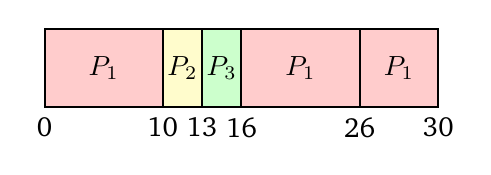
\begin{tikzpicture}[line width=.7pt]
          \draw[fill=red!20] (0,0)node[below]{0} rectangle(1.5,1);
          \draw[fill=yellow!20] (1.5,0)node[below]{10}rectangle(2,1);
          \draw[fill=green!20] (2,0)node[below]{13}rectangle (2.5,1);
          \draw[fill=red!20] (2.5,0)node[below]{16} rectangle(4,1);
          \draw[fill=red!20] (4,0)node[below]{26} rectangle(5,1)node[below,yshift=-1cm]{30};
          
          \path (0.75,.5)node{$P_1$} (1.75,.5)node{$P_2$} (2.25,.5)node{$P_3$} (3.25,.5)node{$P_1$} (4.5,.5)node{$P_1$};
        \end{tikzpicture}
        \end{center}
        \begin{center}
        Average waiting time: $\frac{\color{orange}(10-0) \color{black}+ \color{green}(13-0) \color{black}+ \color{red}(16-10)}{3} = 9\frac{2}{3}$	
        \end{center}
        \end{shaded}
        
 
        
        
        \end{document}
        